\documentclass[12pt]{article}
\usepackage[spanish]{babel}
\usepackage{apacite}
\usepackage[utf8]{inputenc}
\usepackage{amsmath}
\usepackage{newtxtext,newtxmath}
\usepackage{listings}
\usepackage[usenames]{color}
\definecolor{gray97}{gray}{.97}
\definecolor{gray75}{gray}{.75}
\definecolor{gray45}{gray}{.45}
\definecolor{azul1}{RGB}{141,198,163}
\definecolor{azul2}{RGB}{24,107,122}
\definecolor{verde1}{RGB}{44,186,34}
\usepackage{textcomp}
\lstset{
		frame=Ltb,
		framerule=1pt,
		framextopmargin=3pt,
		framexbottommargin=3pt,
		framexleftmargin=0.4cm,
		framesep=0pt,
		rulesep=.4pt,
		backgroundcolor=\color{gray97},
		rulesepcolor=,
        tabsize=4,
        rulecolor=\color{azul1},
        basicstyle=\scriptsize\rmfamily,
        upquote=true,
        aboveskip={1.5\baselineskip},
        columns=fixed,
        showstringspaces=false,
        extendedchars=true,
        breaklines=true,
        prebreak = \raisebox{0ex}[0ex][0ex]{\ensuremath{\hookleftarrow}},
        showtabs=false,
        showspaces=false,
        showstringspaces=false,
        identifierstyle=\rmfamily,
        keywordstyle=\color[rgb]{0,0,1},
        commentstyle=\color[rgb]{0.133,0.545,0.133},
        stringstyle=\color[rgb]{0.627,0.126,0.941},
        keywordstyle=\bfseries,
		numbers=left,
		numbersep=15pt,
		numberstyle=\tiny,
		numberfirstline = false,
		breaklines=true,
		}
\usepackage{graphicx}
\usepackage[colorinlistoftodos]{todonotes}
\usepackage{natbib} %citas bibliograficas estilo APA :p
\usepackage{eso-pic}
\usepackage{avant}
\usepackage[top=2cm,bottom=2cm,left=2.5cm,right=3cm,headsep=8pt,a4paper]{geometry}
\usepackage{fancyhdr}
\pagestyle{fancy}
\fancyhf{}
%\fancyhead[LE,RO]{}
\fancyhead[RE,LO]{Robótica}
\fancyfoot[CE,CO]{\leftmark}
\fancyfoot[LE,RO]{\thepage}
\renewcommand{\headrulewidth}{2pt}
\renewcommand{\footrulewidth}{1pt}
\usepackage{tabu}
\usepackage{array}
\usepackage{multirow}
\usepackage{amssymb}
\usepackage{makeidx}
\graphicspath{ {images/} }
\usepackage{wrapfig}
\usepackage{enumerate}
\usepackage{amsmath,tikz}
\usetikzlibrary{matrix}
\usepackage{steinmetz}
\newcommand*{\horzbar}{\rule[0.05ex]{2.5ex}{0.5pt}}
\usepackage{calc}
\date{\today}


\begin{document}

\begin{titlepage}
\newcommand{\HRule}{\rule{\linewidth}{0.5mm}} 
\center
\textsc{\LARGE  Benemérita Universidad \\[0.2cm] Autónoma de Puebla}\\[1.5cm] 

\includegraphics[width=4cm]{IMAGENES/escudo}\\[1cm]
\textsc{\Large Facultad de Ciencias de la Electrónica}\\[0.5cm] 
\textsc{\large Licenciatura en Electrónica}\\[0.5cm]
\HRule \\[0.4cm]
{ \huge \bfseries Preliminares Matemáticos}\\[0.4cm] 
\HRule \\[1.5cm]
\begin{minipage}{\textwidth}
\center 
\textsc{\LARGE Robótica}\\[1.7cm] 
\emph{Profesor:} \\
Dr. Fernando Reyes Cortés \\[1cm]
\begin{tabular}{ll}
\emph{Alumno:} & \emph{Número de Matrícula:}\\
Hanan Ronaldo Quispe Condori  & 555010653\\
\end{tabular}
\end{minipage}\\[2cm]
\today
\end{titlepage}

\newpage
\section{Introducción}
En el presente informe se desarrollaran soluciones mediante el software de MATLAB para sistemas dinámicos ademas de ello, se presentará un análisis cualitativo de los datos obtenidos 
en el laboratorio de robótica.\vspace{4mm}
\\ 
Estos sistemas dinámicos son modelos matemáticos de ecuaciones diferenciales que describen fenomenos físicos que se encuentren presentes en 
el robot[\cite{reyes2011robotica}].\vspace{4mm} 
\\
Haremos un análisis de las características cualitativas del punto de equilibrio del sistema dinámico(ecuación en lazo cerrado formada por la dinámica del péndulo-robot y el algoritmo de control)
,esto con la ayuda de los datos obtenidos del experimento realizado en el laboratorio.\vspace{4mm}
\\
Se verá que la implementación del código presentado en clase hizo más rapido el proceso de simulación y resolución de los problemas planteados, esto solo se pudo lograr luego de 
una compresión de los mismos.\vspace{4mm}
\\
Cada solución ofrecida a los problemas se dará de la manera 
más clara posible tal y como se afronto en la realización de los mismos.\vspace{4mm}
\\ 
Este informe consta de los siguientes apartados

\begin{itemize}
    \item Introducción
    \item Propositos
    \item Descripción del Problema
    \item Solución del Problema
    \item Resultados
    \item Conclusiones
\end{itemize}

Todos estos apartados se desarrollarán de la manera más concisa relacionada al problema propuesto.\vspace{4mm} 
\\
La solución mediante MATLAB es de gran utilidad, este al ser un lenguaje de alta complejidad permite una variedad de herramientas a la hora de resolver problemas y comprobación de resultados con fiabilidad, bastante
precisión y en tiempos cortos. \vspace{4mm} 
\\
En los anexos se adjuntarán los codigos en su totalidad para su revisión y los gráficos generados por estos que nos permitiran tener una mayor compresión de los sistemas dinámicos planteados.\vspace{4mm}
\\
Finalmente, en el apartado de conclusiones se hara un balance de los puntos importantes que conllevo la realización del presente informe, habrá especial enfoque en la metodología empleada para la implementación del código.\vspace{4mm}
\\ 
De igual manera en el apartado de refercias se podrán encontrar mayor información con respecto a los temas de sistemas dinámicos y punto de equilibrio de un sistema dinámico.

\section{Propositos}
Los objetivos esperados son los siguientes
\begin{itemize}
    \item Interpretar  el punto de equilibrio del sistema dinámico usando los datos experimentales obtenidos en el laboratorio de robótica
    \item Usar el software de MATLAB para solucionar el sistema dinámico propuesto, haciendo uso de los distintos metodos presentados en sesión de clase.
\end{itemize}
\section{Descripción del Problema}
\begin{enumerate}
    \item Explicar cualitativamente la interpretación física del punto de equilibrio de un sistema dinámico(ecuación en lazo cerrado formada por la dinámica del péndulo-robot y el algoritmo de control).
    \item Considere el achivo experimental denominado robot.dat, el cual contiene la información experimental en cuatro columnas; primera columna corresponde al tiempo real, segunda columna posición articular $q(t_k)$[grados];la velocidad de movimiento $\dot{q}(t_k)$[grados/segundo]. Finalmente, la cuarta columna registra el par $\tau$[Nm] aplicado al motor cada columna consta de 2000 reglones; el periodo de muestreo es de 2.5mseg
    \begin{enumerate}
        \item Describir la energía mecánica aplicada a la ecuación en lazo cerrado $V(\dot{q},\tilde{q})$(graficar y analizar resultados).
        \item  Describir la potencia mecánica de la ecuación en lazo cerrado $V(\dot{q},\tilde{q})$(graficar y analizar resultados).
    \end{enumerate} 
    \item Considere la siguiente ecuación diferencial
    \begin{equation}
        \begin{split}
            9\dddot{y}+8\ddot{y}+0.23\dot{y}+\pi y&=3u\\
        \end{split}
        \label{eq:ode}
    \end{equation}
    Donde la entrada $u$ es el escalon unitario.
    \begin{enumerate}
        \item Realice la simulación del sistema con la función ode45().
        \item Resuelva numéricamente el sistema dinámico usando el metodo de Euler.
        \item Resuelva numéricamente el sistema dinámico usando el metodo de filtrado.
        \item Lleve a cabo una comparación de los metodos numéricos utilizados.
    \end{enumerate}
\end{enumerate}
\section{Solución del Problema}
\begin{enumerate}
    \item En un sistema dinámico el punto de equilibrio tiene la caracteristica de ser un atractor, al existir una perturbación de magnitud acotada y tiempo finito, será atrapado por el punto de equilibrio haciendo que el error $\tilde{q}=q_d-q$ sea cero, esto quiere decir que el robot alcanzo la posición deseada, en este punto la velocidad y la energia tambien serán cero ya que al ser la energia una función de Lyapunov, evaluada en el punto de equilibrio es cero, esta es una caracteristica del punto de equilibrio.
    %\vspace{10mm}
    \item 
    \begin{enumerate}
        \item Sea la ecuación dada del torque aplicado
        \begin{equation}
            \begin{split}
                \tau_c&=k_p atanh(\tilde{q})-k_v atan(\dot{q})+mlsen(q)\\
            \end{split}
            \label{eq:torq}
        \end{equation}
        Sea el modelo dinámico del péndulo[\cite{reyes2011robotica}].
        \begin{equation}
            \begin{split}
                \tau_c&=I\ddot{q}+b\dot{q}+mlsen(q)\\
            \end{split}
            \label{eq:pendulo}
        \end{equation}
        La ecuación en lazo cerrado estará dada por 
        \begin{equation}
            \begin{split}
                k_p atanh(\tilde{q})-k_v atan(\dot{q})&=I\ddot{q}+b\dot{q}\\
                \ddot{q}&=\frac{1}{I}(k_p atanh(\tilde{q})-k_v atan(\dot{q})-b\dot{q})\\
                \tilde{q}&=q_d-q\\
                \dot{\tilde{q}}&=-\dot{q}\\
            \end{split}
            \label{eq:close_loop}
        \end{equation}
        Ordenando las ecuaciones \ref{eq:close_loop} se tiene
        \begin{equation}
            \begin{split}
                \frac{d}{dt}
                \begin{bmatrix}
                    \tilde{q} \\
                    \dot{q}
                \end{bmatrix}&=
                \begin{bmatrix}
                    -\dot{q}\\
                    \frac{1}{I}(k_p atanh(\tilde{q})-k_v atan(\dot{q})-b\dot{q})
                \end{bmatrix}\\
            \end{split}
            \label{eq:din_model}
        \end{equation}
        Se propondra la siguiente función de energia
        \begin{equation}
            \begin{split}
                V(\dot{q},\tilde{q})&=\frac{1}{2}I\dot{q}^2+b+\frac{1}{2}k_p\tilde{q}^2-\frac{e_0\tilde{q}\dot{q}I}{1+\tilde{q}^2}\\
            \end{split}
            \label{eq:energia}
        \end{equation}
        El error esta definido como la diferencia entre la posición deseada y la posición actual, bajo esta premisa de los datos obtenidos en el laboratorio se tendrá
        \lstinputlisting[language=Matlab]{Matlab/extraccion.m}
        

        Graficando el error vs la velocidad se tendrá
        %\vspace{100mm}

        \begin{figure}[h]
            \centering
            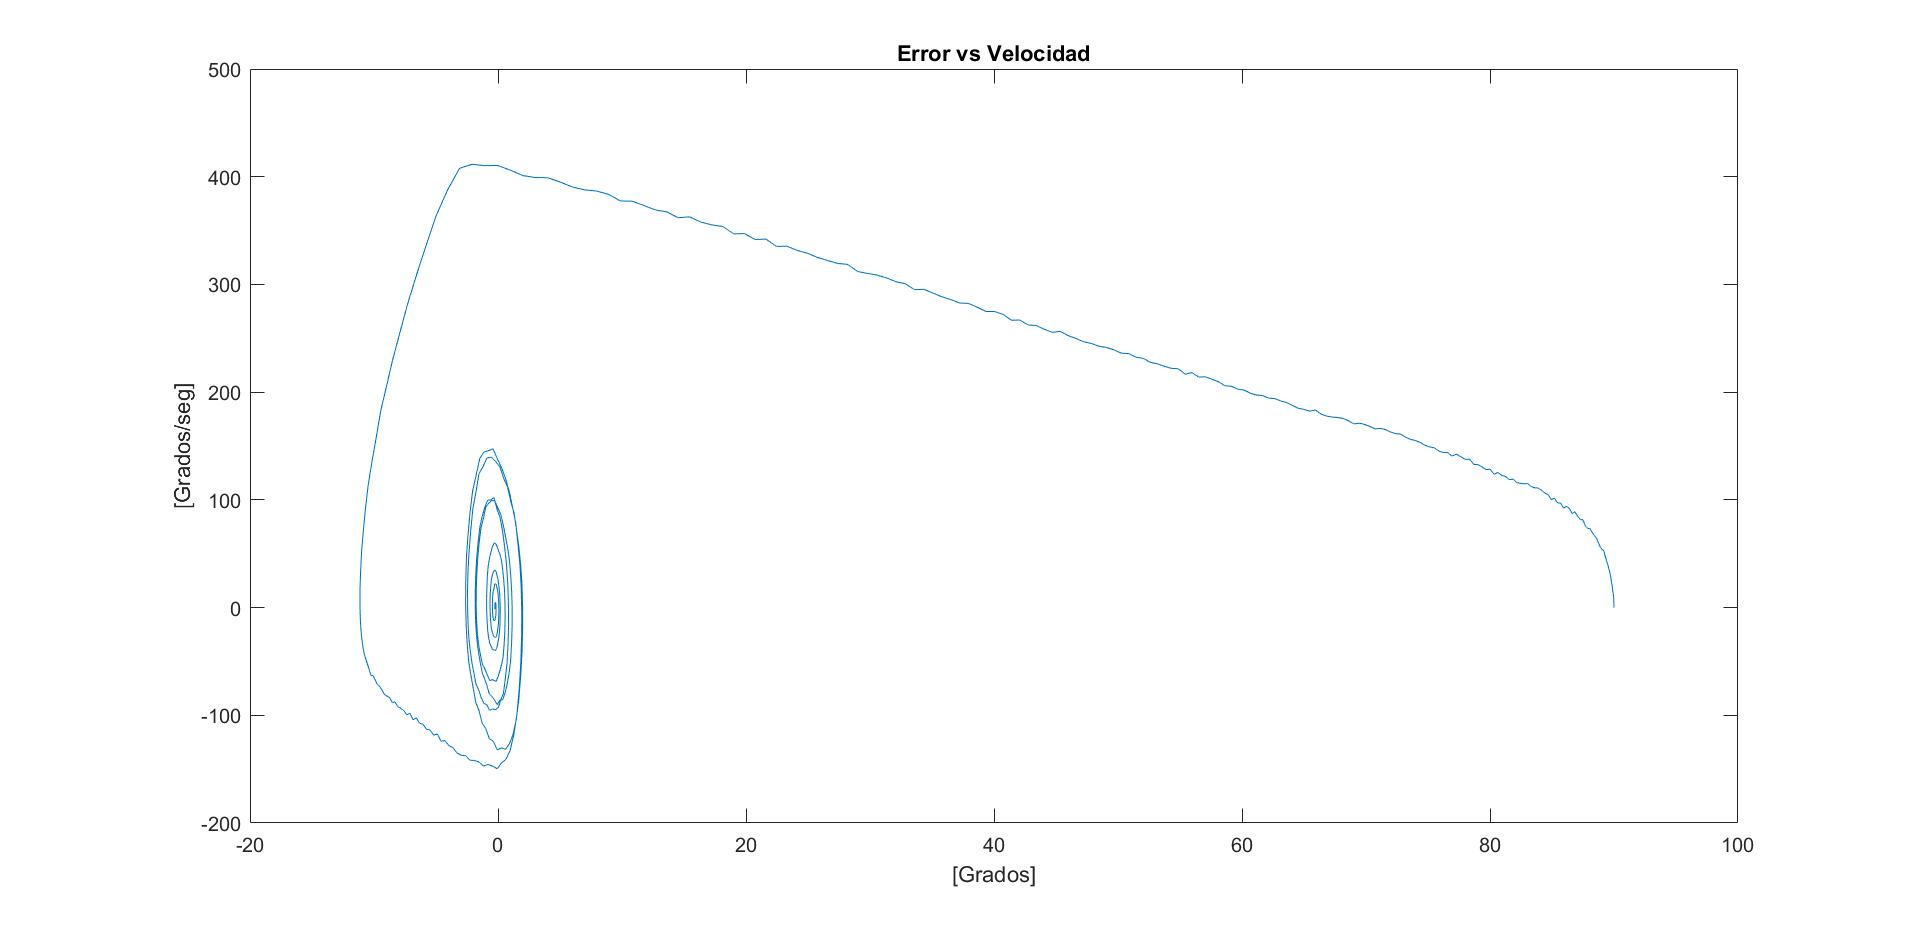
\includegraphics[width=15cm, height=7cm]{IMAGENES/5.jpg}
            \caption{Energia Mecánica Aplicada al Sistema.}
            \label{fig:energia}
        \end{figure}

        La figura \ref{fig:energia} nos muestra el comportamiento del error y la velocidad de nuestro sistema, se puede observar que ambos convergen en cero a medida que pasa el tiempo, esto es una comprobación de que han llegado al punto de equilibrio, por caracteristica del punto de equilibrio en este punto el error es cero ya que se llego a la posición deseada y la velocidad en este punto tambien es cero.
        
        \item
        De las ecuaciones \ref{eq:din_model} y \ref{eq:energia} la potencia mecánica estará dada por
        \begin{equation}
            \begin{split}
                \dot{V}(\dot{q},\tilde{q})=-1\lbrack\dot{q}^2(b+2e_0I-\frac{e_0I}{1+\tilde{q}^2})+\tilde{q}\dot{q}\lbrack k_p-\frac{e_0b}{1+\tilde{q}^2}) \rbrack+(\dot{q}-\frac{e_0\tilde{q}}{1+\tilde{q}^2})\\(k_v atanh(\dot{q})-k_p atan(\tilde{q})) \rbrack\\
            \end{split}
            \label{eq:potencia}
        \end{equation}
        Graficando con los datos del laboratorio se tendrá
        
        \begin{figure}[h]
            \centering
            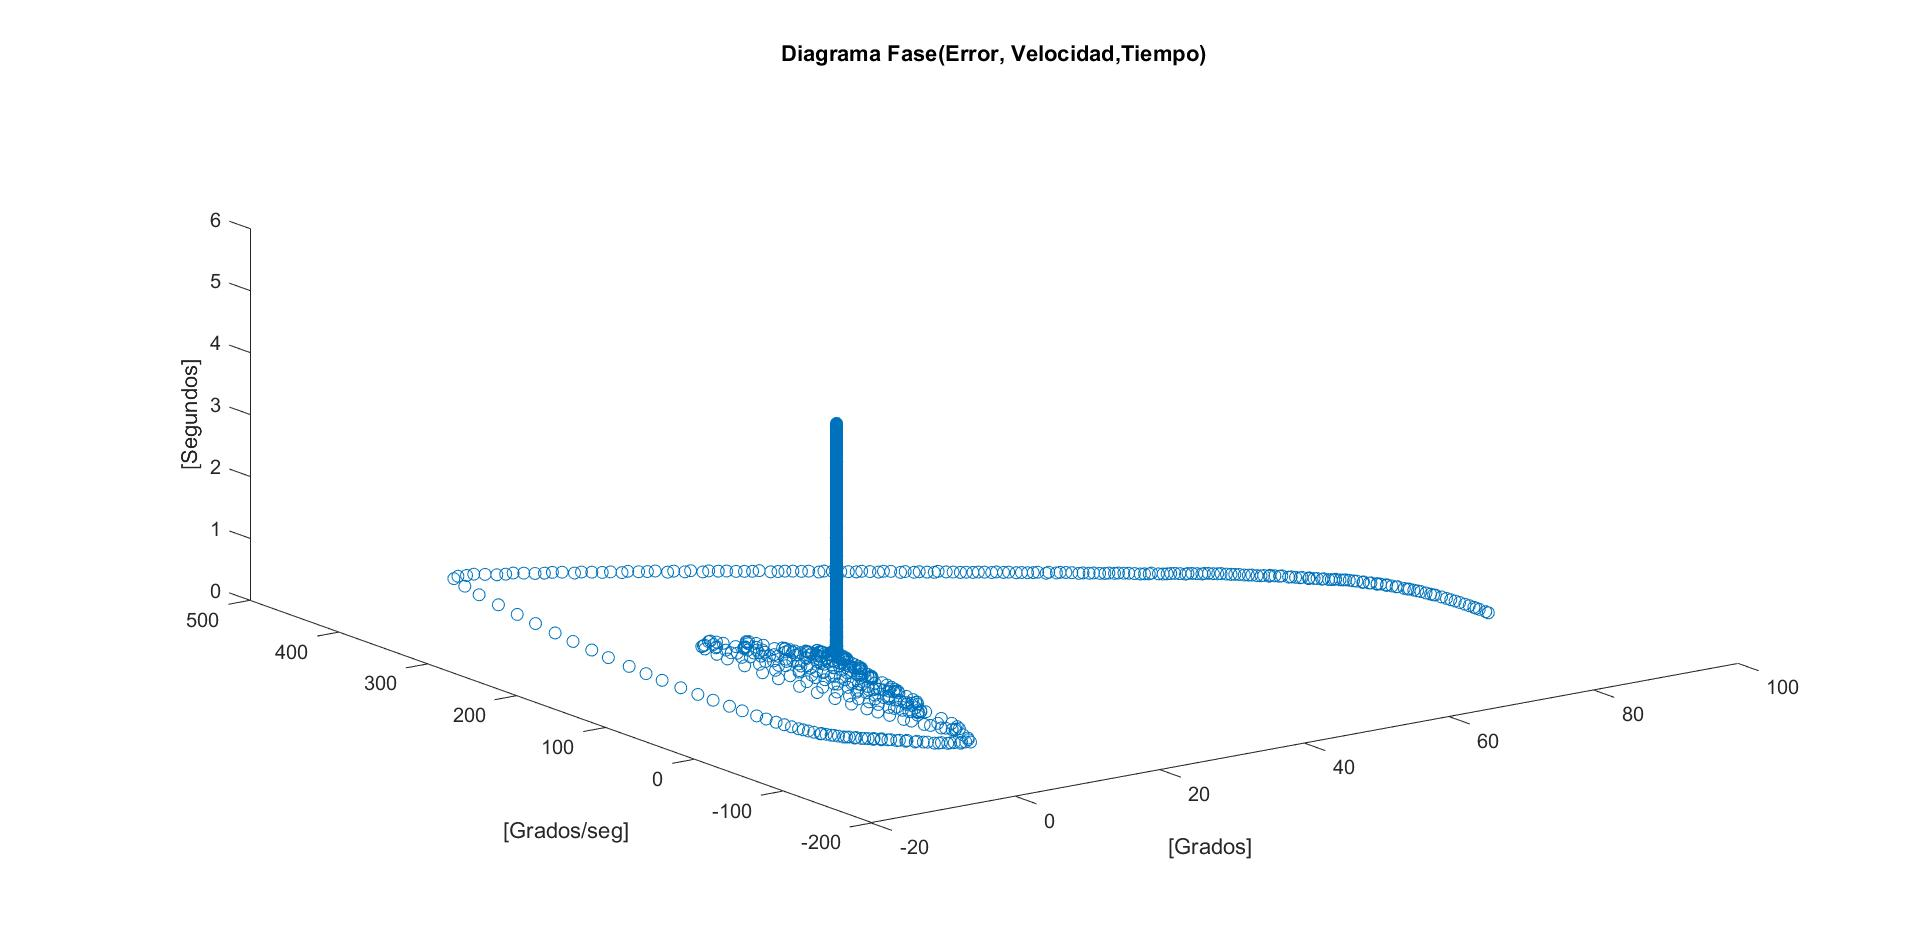
\includegraphics[width=15cm, height=7cm]{IMAGENES/6.jpg}
            \caption{Potencia Mecánica Aplicada al Sistema.}
            \label{fig:potencia}
        \end{figure}
        
        La figura \ref{fig:potencia} nos muestra como evoluciona la energia con respecto pasa el tiempo, se puede observar claramente que una vez el punto de equilibrio es alcanzado, la energia se hace cero, al igual que la velocidad y el error[\cite{Lyapunov}].
    \end{enumerate}
    \item Usaremos MATLAB para obtener el modelo dinámico de la ecuación dada.
    
    \lstinputlisting[language=Python]{Matlab/diary}
        
    %\begin{figure}[h]
    %    \centering
    %    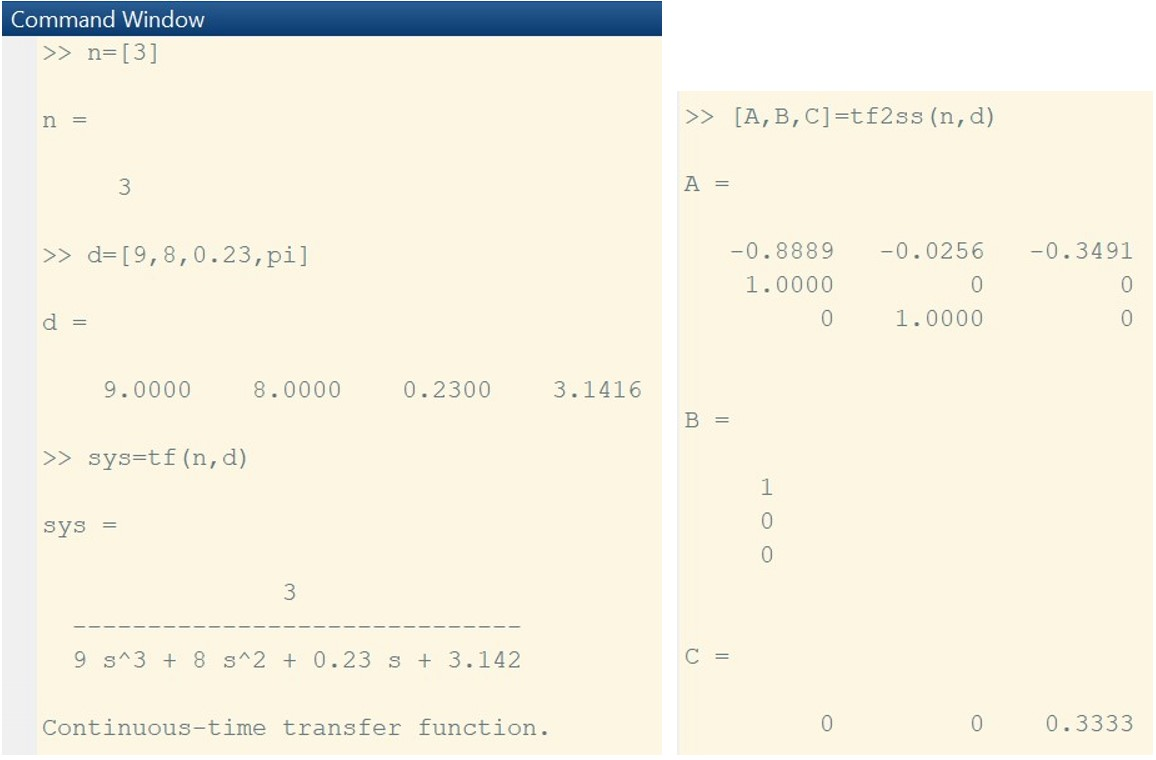
\includegraphics[width=8cm]{IMAGENES/8.jpg}
    %    \caption{Obtención del modelo dinámico.}
    %\end{figure}
    Primero se usara la función "tf" para obtener la función de transferencia del sistema despues usaremos la función "tf2ss" para obtener el modelo dinámico del sistema.
    \begin{enumerate}
        \item Se usaran las matrices A y B como se muestra a continuación.
        
        \lstinputlisting[language=Matlab]{Matlab/sso.m}
        
        La función principal es
        \lstinputlisting[language=Matlab]{Matlab/simul_matrix.m}

        El resultado obtenido es
        \begin{figure}[h]
            \centering
            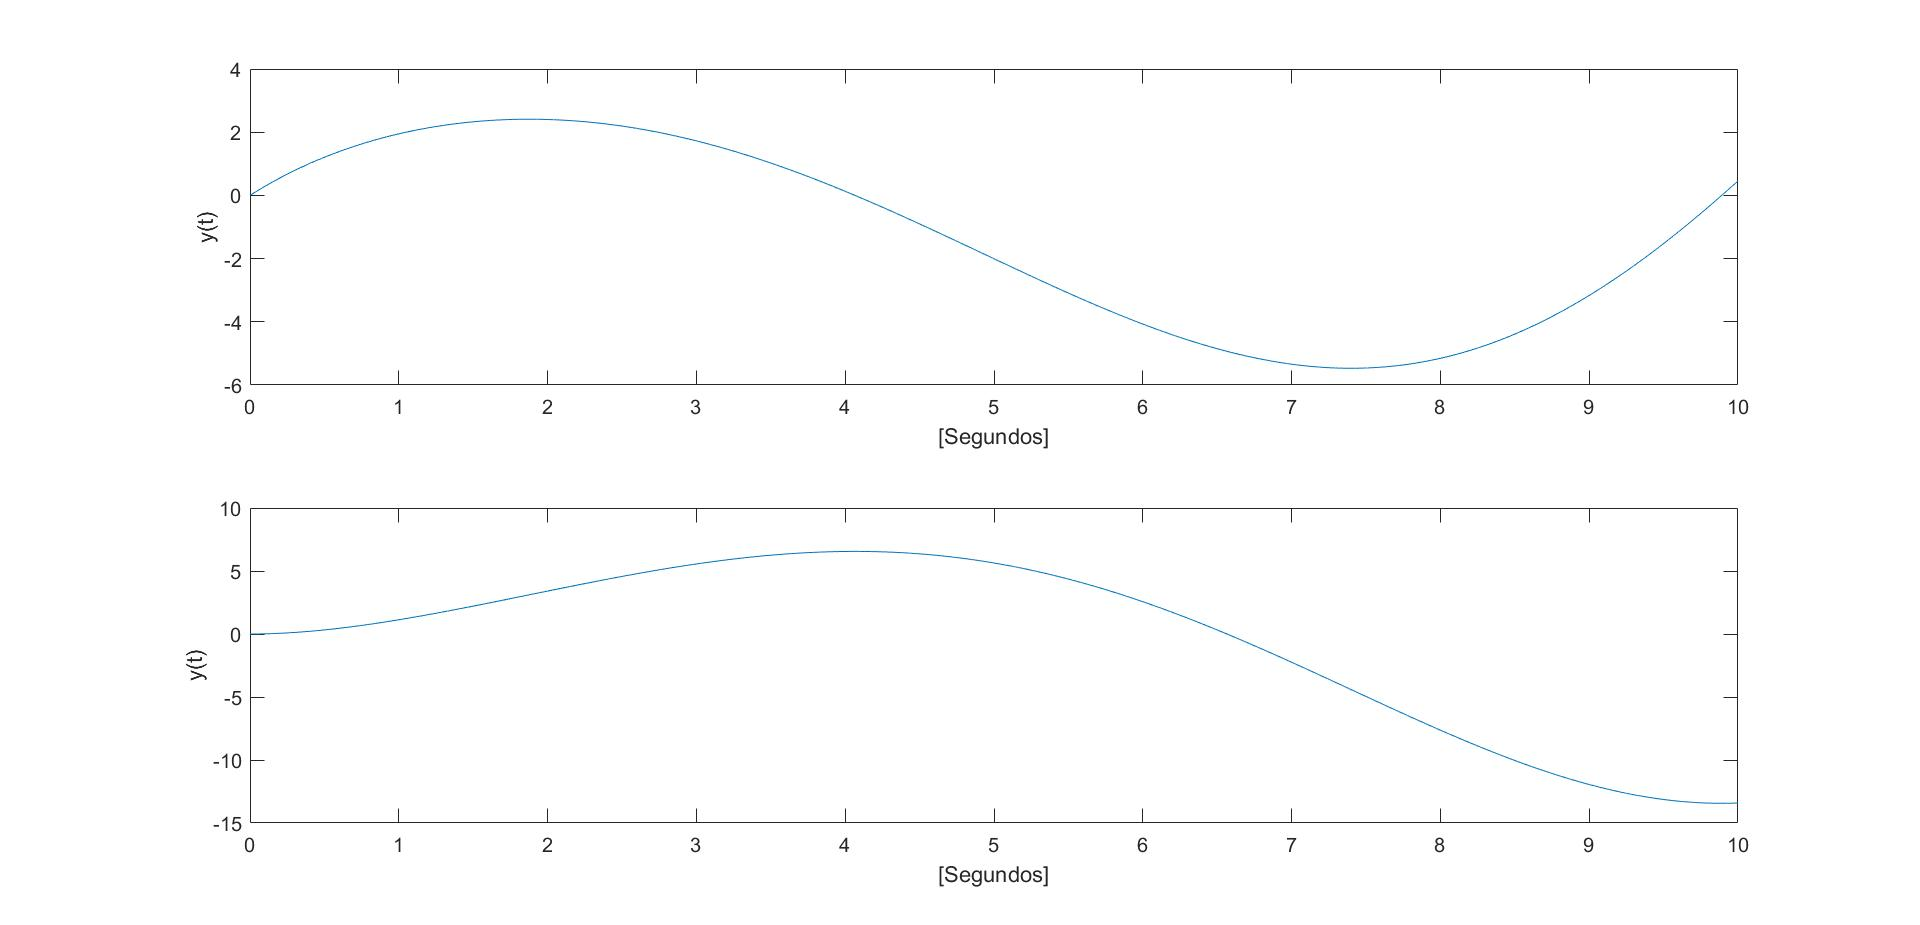
\includegraphics[width=15cm]{IMAGENES/9.jpg}
            \caption{Simulación por ode45.}
        \end{figure}
        
        La función ode45 retorna la solución del sistema asi como el vector de tiempo.
        \item 
    \end{enumerate}
    %\vspace{50mm}
\end{enumerate}
\section{Resultados}
\section{Conclusiones}
\section{Anexos}
\bibliographystyle{apacite}
\bibliography{biblio}
\end{document}